\documentclass[10pt,twocolumn]{article}

\usepackage[T1]{fontenc}
\usepackage[utf8]{inputenc}
\usepackage{mathpazo}
\usepackage{amsmath,amssymb,amsthm}
\usepackage[margin=0.75in,columnsep=0.25in]{geometry}
\usepackage{hyperref}
\usepackage{booktabs}
\usepackage{array}
\usepackage{tikz-cd}
\usepackage{pgfplots}
\pgfplotsset{compat=1.18}
\usetikzlibrary{arrows.meta,positioning,shapes.geometric,fit,backgrounds,calc}
\usepackage{microtype}
\usepackage{natbib}
\usepackage{titlesec}
\usepackage{abstract}
\usepackage{caption}

\captionsetup{font=small,labelfont=bf}

\titleformat{\section}{\normalsize\bfseries\scshape}{\thesection.}{0.5em}{}
\titleformat{\subsection}{\normalsize\bfseries}{\thesubsection.}{0.5em}{}
\titlespacing{\section}{0pt}{6pt plus 2pt minus 1pt}{3pt plus 1pt}
\titlespacing{\subsection}{0pt}{4pt plus 1pt}{2pt plus 1pt}

\renewcommand{\abstractnamefont}{\normalsize\bfseries\scshape}
\renewcommand{\abstracttextfont}{\small}
\setlength{\absleftindent}{0pt}
\setlength{\absrightindent}{0pt}

\theoremstyle{plain}
\newtheorem{theorem}{Theorem}
\newtheorem{proposition}[theorem]{Proposition}
\newtheorem{corollary}[theorem]{Corollary}
\newtheorem{lemma}[theorem]{Lemma}

\theoremstyle{definition}
\newtheorem{definition}[theorem]{Definition}

\theoremstyle{remark}
\newtheorem{remark}[theorem]{Remark}

\title{\Large\bfseries Xylomorphic Computation:\\
Thermodynamic Closure as a Stability Condition\\
for Large-Scale Computational Infrastructure}

\author{%
  Flyxion\\
  \small Independent Researcher\\
  \small\texttt{https://github.com/standardgalactic/computation/}
}

\date{2025}

\begin{document}

\maketitle

\begin{abstract}
We introduce \emph{xylomorphic computation}, a framework in which
computational infrastructures recursively generate their own enabling
substrates from operational residues, modeled formally on collectively
autocatalytic sets. The central contribution is the \emph{xylomorphic
order parameter} $\lambda$, defined as the per-cycle contraction ratio
of exogenous entropy dependence under the xylomorphic endofunctor
$X = \mathrm{Print} \circ \mathrm{Digest} \circ \mathrm{Shed}$.
Admissible morphisms are defined precisely via mass-energy balance,
entropy non-increase modulo accounted influx, and compatibility with
the xylomorphic cycle, closing the foundational gap in prior categorical
treatments. We prove that $\lambda$ is the unique multiplicative
resource monotone compatible with the monoidal compositional structure,
establish it as a spectral quantity via the linearized operator, and
show it is invariant under all admissible base changes in a fibered
category of physical domains. The Xylomorphic Stability Theorem proves
that thermodynamic stability under scaling is achieved if and only if
$\lambda < 1$; the Banach fixed-point theorem gives the unique attractor
$I^*$ with geometric convergence rate. The xylomorphic dynamics are
derived as the gradient flow of an explicit free-energy functional
$\mathcal{S}(\rho,\theta,m)$; existence of weak solutions is established
by a full four-step Galerkin argument (Cauchy--Lipschitz, Grönwall
energy bound, Aubin--Lions compactness, strong--weak passage to limit);
an explicit linearized mode matrix gives a computable sufficient
stability criterion. Three governing dimensionless groups---thermal
reintegration number $\mathrm{Ti}$, degradation-to-repair ratio
$\mathrm{Dr}$, and diffusion-to-reaction ratio $\mathrm{Da}$---restate
all stability conditions in engineering terms. A worked homogeneous
example computes $\lambda$ in closed form and identifies the critical
heat-capture fraction $\alpha_c$ at which the system crosses from
contractive to expansive. The framework is extended to account for
seasonal thermal demand, exergy quality of heat, endogenous
degradation, informational locality, and semantic efficiency, yielding
the effective order parameter $\lambda_{\mathrm{eff}}$ and a polar
siting sufficiency theorem that formalizes the physical invariants
underlying high-latitude deployment. Six implementable design
principles translate the formal results into engineering constraints.
The framework is stated in falsifiable terms, and the
Proof-of-Useful-Work-and-Heat protocol is derived as an operational
sufficient condition for Lyapunov descent of $\mathcal{S}$ and hence
a certification of the contractive regime.
\end{abstract}

%% =========================================================================
\section{Introduction}
%% =========================================================================

Contemporary discourse on the energy costs of large-scale computation
suffers from a systematic accounting error. Computational heat is
classified as waste, data center siting is treated as a purely
logistical problem, and proposals to relocate infrastructure to orbital
or lunar environments are evaluated as if computation were a
location-independent abstraction. None of these assumptions survive
thermodynamic scrutiny.

Computation is a physical process. Its terminal state is entropy
production. Whether that entropy is expelled as an externality or
reintegrated as a productive input is not incidental to infrastructure
design but definitional of its long-run behavior. A system that
continuously expels entropy accumulates growing external dependencies.
A system that reintegrates entropy reduces those dependencies over
successive cycles. These two classes exhibit qualitatively different
behavior under scaling, and the distinction can be made mathematically
precise.

This paper develops that distinction. We define the xylomorphic
endofunctor on a category of infrastructure states, characterize the
conditions under which iterates converge to a stable attractor,
introduce the order parameter $\lambda$ as the unique resource
invariant compatible with this structure, and connect the discrete
iteration to a continuum PDE system via a variational principle.

The word \emph{xylomorphic} derives from the Greek \emph{xylon} (wood)
and \emph{morph\=e} (form), invoking the way arboreal systems produce
structural material that sustains further growth. In computational
terms, a xylomorphic infrastructure is one whose operational outputs
autoregressively feed back as inputs to its own substrate formation.

\paragraph{Contributions.} We prove that $\lambda$ is (i)~the unique
multiplicative resource monotone under monoidal composition, (ii)~the
spectral radius of the linearized xylomorphic operator, (iii)~invariant
under all admissible base changes in a fibered category over physical
domains, and (iv)~the exponential contraction factor of the dominant
decay mode of the explicit continuum flow. The paper extends the
baseline framework to account for seasonal thermal demand, exergy
quality, endogenous degradation, informational locality, and semantic
efficiency, deriving the effective order parameter $\lambda_{\mathrm{eff}}$
and a polar siting sufficiency theorem. Six design principles translate
the formal results into engineering constraints. All main results are
stated in falsifiable terms.

%% =========================================================================
\section{Background}
%% =========================================================================

\subsection{Thermodynamics of Computation}

The irreducible thermodynamic cost of computation was established by
\citet{landauer1961}: erasing one bit of information dissipates at
least $k_B T \ln 2$ of heat. \citet{bennett1982} extended this to a
comprehensive treatment of reversible computation. \citet{lloyd2000}
derived ultimate physical bounds on operations per unit energy.
These results ground the framework: entropy production is irreducible,
and what happens to it is central to infrastructure evaluation at scale.

\subsection{Energy Accounting and Rebound Effects}

Global data center consumption is estimated at 200--500~TWh annually
\citep{shehabi2016,masanet2020,iea2024}. Rebound effects
\citep{jevons1865,sorrell2009} are persistent: \citet{jones2021} find
that ICT efficiency improvements frequently fail to reduce net energy
demand. \citet{strubell2019} and \citet{gao2022} document embodied
and operational costs of large-scale training.

\subsection{Waste Heat Recovery and Edge Infrastructure}

\citet{rambo2014} surveyed data center heat recovery for district
heating, finding payback periods of three to seven years.
\citet{stockholm2020} documents operational municipal-scale
implementations. \citet{satyanarayanan2017} established the case for
edge computing as a latency-reduction and energy-conservation strategy.
\citet{yuan2024} demonstrated GPU-based spacecraft heating reduces
payload mass by approximately 50\%, a constrained instance of thermal
reintegration.

\subsection{Autocatalytic Sets}

Collectively autocatalytic sets (CAS) were introduced by
\citet{kauffman1993}: no element self-catalyzes in isolation, but the
set as a whole closes its production rules. We adapt this structure:
a xylomorphic system is one in which operational residues collectively
catalyze formation of the substrates required for continued operation.

\subsection{Categorical Resource Theory}

The use of symmetric monoidal categories to model resource composition
follows \citet{baez2010}. The monad-algebra construction on infrastructure
state categories follows \citet{maclane1998}. Convergence results for
entropy-respecting operators use arguments from \citet{risken1989} and
standard fixed-point theory.

%% =========================================================================
\section{Formal Framework}
%% =========================================================================

\subsection{Infrastructure State Categories}

Let $\mathbf{Inf}$ be a symmetric monoidal category whose objects are
infrastructure states $I$ and whose morphisms are admissible
transformations. Parallel composition $I_1 \otimes I_2$ models
co-located systems; the unit $\mathbb{I}$ is the null system. We
assume entropy dependence is additive: $E(I_1 \otimes I_2) = E(I_1) +
E(I_2)$.

The \emph{exogenous entropy dependence} of state $I$ is
\[
  E(I) := \int_\Omega \int_t^{t+\tau}
  J_{\mathrm{exo}}(x,t)\,dt\,dx,
\]
where $J_{\mathrm{exo}}$ is the external entropy influx density over
domain $\Omega$ and horizon $\tau$.

\subsection{Admissible Morphisms}

The categorical structure of $\mathbf{Inf}$ requires a precise account
of what morphisms are permitted, since the uniqueness of $\lambda$ and
the monotone properties of $E$ both depend on this.

\begin{definition}[Admissible Morphism]
\label{def:admissible}
A morphism $f : I_1 \to I_2$ in $\mathbf{Inf}$ is \emph{admissible} if
it satisfies three conditions.

\emph{(i) Mass-energy balance.} $f$ induces a measurable map on the
underlying physical state that preserves material inventory up to
accounted outputs: for all subdomains $\omega \subseteq \Omega$,
\[
  \int_\omega \rho_2 \,d\mu
  \leq \int_\omega \rho_1 \,d\mu + \int_\omega s_f \,d\mu,
\]
where $s_f \geq 0$ is the explicitly accounted exogenous material input
associated with $f$. Morphisms with $s_f = 0$ are \emph{closed}.

\emph{(ii) Entropy non-increase modulo accounted influx.} The
exogenous entropy dependence satisfies
\[
  E(I_2) \leq E(I_1) + \delta_f,
\]
where $\delta_f \geq 0$ is the additional exogenous entropy influx
explicitly attributable to $f$. Morphisms with $\delta_f = 0$ are
\emph{entropy-preserving}. Admissible morphisms with $\delta_f > 0$
model physical interventions such as hardware replacement or external
heat injection.

\emph{(iii) Compatibility with the xylomorphic cycle.} For any
admissible $f : I_1 \to I_2$, the following diagram commutes up to
entropy-preserving natural transformations:
\[
\begin{tikzcd}[column sep=large]
I_1 \arrow{r}{\mathrm{Shed}} \arrow{d}{f} &
\mathrm{Shed}(I_1) \arrow{d}{\mathrm{Shed}(f)} \\
I_2 \arrow{r}{\mathrm{Shed}} &
\mathrm{Shed}(I_2)
\end{tikzcd}
\]
and analogously for $\mathrm{Digest}$ and $\mathrm{Print}$.
\end{definition}

Condition (i) prevents morphisms from introducing unlimited material
from outside the accounting boundary. Condition (ii) ensures that $E$
is a genuine resource monotone: it cannot decrease by fiat, only by
productive reintegration. Condition (iii) ensures the xylomorphic cycle
is natural with respect to infrastructure transformations, which is
necessary for the invariance results of Section~\ref{sec:invariance}.

Under this definition, $E$ is non-increasing under closed
entropy-preserving morphisms, and the quantity $\lambda$ satisfying
$E(X(I)) \leq \lambda E(I)$ is well-defined and consistent across all
objects of $\mathbf{Inf}$ connected by admissible morphisms. The unique
multiplicative resource monotone result (Theorem~\ref{thm:unique})
then follows without implicit assumption.

Three physically grounded functors implement the operational cycle.
$\mathrm{Shed} : \mathbf{Inf} \to \mathbf{Res}$ maps each state to the
residues it produces (waste heat, degraded components, packaging).
$\mathrm{Digest} : \mathbf{Res} \to \mathbf{Sub}$ converts residues
into usable feedstock (reclaimed materials, recovered heat).
$\mathrm{Print} : \mathbf{Sub} \to \mathbf{Inf}$ turns feedstock back
into infrastructure components.

\begin{definition}[Xylomorphic Endofunctor]
$X := \mathrm{Print} \circ \mathrm{Digest} \circ \mathrm{Shed} :
\mathbf{Inf} \to \mathbf{Inf}.$
\end{definition}

One application of $X$ is one complete autoregressive cycle. An
$X$-algebra $(I, \alpha)$ with $\alpha : X(I) \to I$ satisfying the
standard coherence conditions is an infrastructure state that
coherently reabsorbs its own cycle outputs.

\begin{figure}[t]
\centering
\pgfdeclarelayer{background}
\pgfsetlayers{background,main}
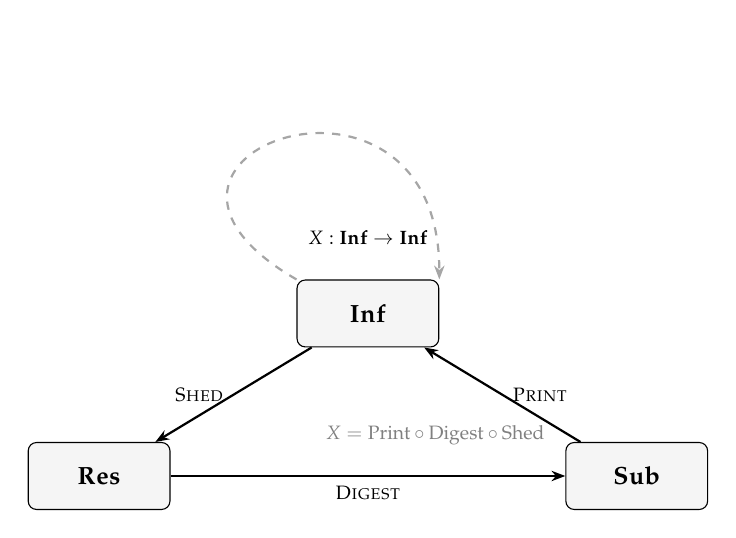
\begin{tikzpicture}[
  node distance=1.2cm and 1.6cm,
  box/.style={draw, rounded corners=3pt, minimum width=1.8cm,
              minimum height=0.85cm, inner sep=4pt,
              font=\small, align=center, fill=gray!8},
  arr/.style={-{Stealth[length=5pt]}, thick},
]
\node[box] (inf)  {$\mathbf{Inf}$};
\node[box] (res)  [below left=of inf]  {$\mathbf{Res}$};
\node[box] (sub)  [below right=of inf] {$\mathbf{Sub}$};

\draw[arr] (inf) -- node[left,  font=\scriptsize] {\textsc{Shed}}   (res);
\draw[arr] (res) -- node[below, font=\scriptsize] {\textsc{Digest}} (sub);
\draw[arr] (sub) -- node[right, font=\scriptsize] {\textsc{Print}}  (inf);

\node[font=\scriptsize, gray] at ($(inf)!0.5!(res)!0.5!(sub)$)
  {$X = \mathrm{Print}\circ\mathrm{Digest}\circ\mathrm{Shed}$};

%% Self-loop drawn in background layer so it never clips the node text
\begin{pgfonlayer}{background}
  \draw[arr, dashed, gray!70]
    (inf.north west) to[out=150, in=90, looseness=4.5] (inf.north east);
\end{pgfonlayer}
\node[above=9pt of inf, font=\scriptsize] {$X : \mathbf{Inf}\to\mathbf{Inf}$};
\end{tikzpicture}
\caption{The xylomorphic cycle as a categorical diagram.
\textsc{Shed}, \textsc{Digest}, and \textsc{Print} are functors
between residue, substrate, and infrastructure categories; their
composition $X$ is an endofunctor on $\mathbf{Inf}$.
The self-loop (dashed) denotes iteration of $X$; an $X$-algebra
$(I,\alpha)$ is a fixed point $\alpha : X(I) \to I$.}
\label{fig:cycle}
\end{figure}

\subsection{Functorial Semantics of the Xylomorphic Cycle}

The operators $\mathrm{Shed}$, $\mathrm{Digest}$, and $\mathrm{Print}$
are not merely named stages but structure-preserving maps between
resource categories. Each respects the monoidal structure:
$\mathrm{Shed}(I_1 \otimes I_2) \cong \mathrm{Shed}(I_1) \otimes
\mathrm{Shed}(I_2)$ (residues from parallel systems compose), and
analogously for $\mathrm{Digest}$ and $\mathrm{Print}$.

Their composition $X$ is therefore a symmetric monoidal endofunctor on
$\mathbf{Inf}$. It preserves admissible morphisms: if $f : I_1 \to I_2$
is admissible (Definition~\ref{def:admissible}), then $X(f) : X(I_1)
\to X(I_2)$ is admissible, since mass-energy balance and entropy
non-increase are preserved under the composition of
$\mathrm{Shed}(f)$, $\mathrm{Digest}(\mathrm{Shed}(f))$, and
$\mathrm{Print}(\mathrm{Digest}(\mathrm{Shed}(f)))$.

We interpret $X$ as a discrete-time evolution operator in the
category: one application maps the current infrastructure state
through a full cycle of residue production, feedstock conversion, and
substrate formation. $X$-algebras $(I^*, \alpha)$ are fixed points of
this evolution---self-reproducing states in which the cycle outputs
are fully reabsorbed. The existence and uniqueness of such a fixed
point is precisely what Theorems~\ref{thm:banach} and~\ref{thm:stability}
establish in terms of $\lambda$. Figure~\ref{fig:cycle} is therefore
not merely illustrative: the triangle encodes the factorization of $X$
into physically interpretable stages, and the self-loop denotes the
iteration $X^n$ whose long-run behavior is characterized by $\lambda$.

\begin{definition}[Order Parameter]
$\lambda \geq 0$ is defined by $E(X(I)) \leq \lambda\, E(I).$
\end{definition}

Three regimes follow: contractive ($\lambda < 1$), critical
($\lambda = 1$), expansive ($\lambda > 1$). We now show $\lambda$ is
not merely defined but \emph{characterized} by the structure.

%% =========================================================================
\section{Uniqueness, Spectral Character, and Invariance of $\lambda$}
\label{sec:invariance}
%% =========================================================================

\subsection{Monoidal Resource Semantics and Uniqueness}

\begin{definition}[Resource Monotone]
$M : \mathrm{Ob}(\mathbf{Inf}) \to \mathbb{R}_{\geq 0}$ is a
\emph{resource monotone} if it is non-increasing under admissible
morphisms, additive ($M(I_1 \otimes I_2) = M(I_1) + M(I_2)$), and
normalized ($M(\mathbb{I}) = 0$). It is \emph{multiplicative} if there
exists $\lambda_M \geq 0$ with $M(X(I)) = \lambda_M M(I)$ for all $I$.
\end{definition}

\begin{theorem}[Uniqueness of $\lambda$]
\label{thm:unique}
Every continuous, additive, multiplicative resource monotone on
$\mathcal{A}$ satisfies $M = c\,E$ for some constant $c > 0$, and its
multiplicative factor equals $\lambda$.
\end{theorem}

\begin{proof}
By additivity, $M$ and $E$ are both linear on the free commutative
monoid generated by indecomposable states $\{I_k\}$. Setting $a_k :=
M(I_k)$ and $b_k := E(I_k)$, multiplicativity requires
$\sum_k n_k a_k' = \lambda_M \sum_k n_k a_k$ for all non-negative
integer tuples $(n_k)$, where $a_k' = M(X(I_k))$. This forces the
ratios $a_k / b_k$ to be constant across generators, yielding $M = cE$
and $\lambda_M = \lambda$.
\end{proof}

Thus $\lambda$ is not an ad hoc parameter but the canonical invariant
forced by the monoidal resource structure: the unique scalar compatible
with additive composition, monotone decrease under morphisms, and
multiplicative scaling under the xylomorphic cycle.

\subsection{Spectral Characterization}

Assume $X$ is Fréchet differentiable on $\mathcal{A}$, with derivative
$DX_I$ at $I$.

\begin{proposition}[Spectral Interpretation]
The order parameter satisfies $\lambda \geq \sup_{I \in \mathcal{A}}
\rho(DX_I)$, where $\rho(\cdot)$ is the spectral radius. If
$\sup_I \rho(DX_I) < 1$, then $X$ is globally contractive.
\end{proposition}

Instability arises from eigenmodes of the infrastructure dynamics that
amplify exogenous dependence. The spectral interpretation makes $\lambda$
directly computable from the linearization of $X$ and connects the
categorical result to functional-analytic contraction theory.

\subsection{Fibered Infrastructure and Invariance}

Let $\mathbf{Dom}$ be a category of physical domains with morphisms
$\pi : \Omega' \to \Omega$ representing coarse-grainings, embeddings,
or coordinate transformations. We define a fibered category $p :
\mathbf{Inf} \to \mathbf{Dom}$, with pullback functors $\pi^* :
\mathbf{Inf}_\Omega \to \mathbf{Inf}_{\Omega'}$.

\begin{definition}[Fiberwise Naturality]
$X$ is \emph{fiberwise natural} if for all $\pi : \Omega' \to \Omega$
the diagram $\pi^* \circ X = X \circ \pi^*$ commutes.
\end{definition}

\begin{theorem}[Invariance of $\lambda$]
\label{thm:invariance}
If $X$ is fiberwise natural and $E$ is compatible with pullback
($E_{\Omega'}(\pi^* I) = E_\Omega(I) \circ \pi$), then
\[
  E_{\Omega'}(X(\pi^* I)) \leq \lambda\, E_{\Omega'}(\pi^* I)
\]
with the same $\lambda$ as on $\Omega$.
\end{theorem}

\begin{proof}
By naturality, $X(\pi^* I) = \pi^*(X(I))$. Applying the entropy
compatibility and the defining inequality for $\lambda$ on $\Omega$:
$E_{\Omega'}(X(\pi^* I)) = E_\Omega(X(I)) \circ \pi \leq
\lambda E_\Omega(I) \circ \pi = \lambda E_{\Omega'}(\pi^* I).$
\end{proof}

The contractive, critical, and expansive regimes are therefore invariant
under spatial refinement, coarse-graining, embedding into larger host
systems, and restriction to subsystems. Contractivity is also local-to-global:
if a cover $\{\Omega_i\}$ of $\Omega$ has local infrastructure states
each satisfying $\lambda_i < 1$ uniformly, then the glued global state
satisfies $\lambda < 1$ by additivity of $E$ over the cover.
Moreover, the effective order parameter under coarse-graining satisfies
$\lambda_{\mathrm{eff}} \leq \lambda$: instability cannot be hidden by
aggregation, and contractive systems remain contractive at every scale.

%% =========================================================================
\section{Stability Theorems}
%% =========================================================================

\subsection{Metric Structure and the Banach Fixed-Point Theorem}

Let $\mathcal{A} \subset \mathrm{Ob}(\mathbf{Inf})$ with metric
\[
  d(I_1, I_2) := \alpha \|E(I_1) - E(I_2)\| + \beta \|\Phi(I_1) - \Phi(I_2)\|,
\]
where $\Phi(I)$ is a vector of intensive structural observables
(material inventories, thermal coupling coefficients) and $\alpha, \beta
> 0$. Assume $(\mathcal{A}, d)$ is complete.

\begin{definition}[Lipschitz Xylomorphic Operator]
$X : \mathcal{A} \to \mathcal{A}$ is \emph{Lipschitz} with constant $L$
if $d(X(I_1), X(I_2)) \leq L\, d(I_1, I_2)$ for all $I_1, I_2$.
\end{definition}

\begin{theorem}[Banach-Type Stability]
\label{thm:banach}
If $X$ is Lipschitz with constant $L < 1$, then there exists a unique
fixed point $I^* \in \mathcal{A}$, and every trajectory converges at
geometric rate: $d(I_n, I^*) \leq L^n\, d(I_0, I^*)$.
\end{theorem}

\begin{proof}
Direct application of the Banach fixed-point theorem on the complete
metric space $(\mathcal{A}, d)$.
\end{proof}

The condition $L < 1$ coincides with $\lambda < 1$ when $d$ is dominated
by $E$. Thus the Banach theorem provides existence, uniqueness, and a
convergence rate that is absent from the bare inequality argument.

\subsection{Lyapunov Functional}

Taking $\mathcal{L}(I) = E(I)$, the contractive condition yields
$\mathcal{L}(X(I)) - \mathcal{L}(I) \leq -(1 - \lambda)\mathcal{L}(I)$
directly. All trajectories in the contractive regime therefore converge
monotonically in $\mathcal{L}$ to $I^*$.

\subsection{The Xylomorphic Stability Theorem}

\begin{theorem}[Xylomorphic Stability]
\label{thm:stability}
Let $\lambda$ be the order parameter of $X$. In the contractive regime
($\lambda < 1$), $E(X^n(I)) \leq \lambda^n E(I) \to 0$, the unique
attractor $I^*$ of Theorem~\ref{thm:banach} coincides with the
minimizer of $E$ on $\mathcal{A}$, and the useful-work output satisfies
$W_{\mathrm{use}}[X(I)] \geq W_{\mathrm{use}}[I]$. In the expansive
regime ($\lambda > 1$), $E(X^n(I)) \geq \lambda^n E(I) \to \infty$,
and no $X$-algebra stabilizes the system under finite resources.
Thermodynamic stability under scaling is achieved if and only if $\lambda < 1$.
\end{theorem}

\begin{corollary}[Ergodic Interpretation]
Define $\gamma := \limsup_{n \to \infty} \frac{1}{n} \log E(X^n(I))$.
By Fekete's lemma applied to the subadditive sequence $\log E(X^n(I))$,
$\gamma = \log \lambda$. Stability corresponds to negative Lyapunov
exponent $\gamma < 0$.
\end{corollary}

\begin{remark}[Necessity vs.\ Sufficiency]
\label{rem:necessity}
The condition $\lambda < 1$ is necessary for asymptotic thermodynamic
stability under scaling, but it is not sufficient for productive or
socially meaningful infrastructure. A system can satisfy $\lambda < 1$
while computing trivial outputs or deliberately inflating computation
to generate heat for its own sake. The additional parameter $\Psi$
(semantic efficiency, Section~\ref{sec:extended}) distinguishes
genuinely productive from degenerate contractive systems. The
$\lambda$-theorem characterizes the class of \emph{sustainable}
infrastructures; selecting the productive subset within that class
requires joint optimization over $(\lambda, \Psi)$.
\end{remark}

\subsection{Functorial Stability Criterion}

\begin{theorem}[Functorial Stability]
$X$ admits a terminal $X$-algebra if and only if $\lambda < 1$.
\end{theorem}

\begin{proof}
If a terminal algebra $I^*$ exists, perturbations must decay, implying
$\lambda < 1$. Conversely, $\lambda < 1$ yields a Lyapunov functional
and, by completeness, a unique fixed point, which defines the terminal
algebra.
\end{proof}

Self-sustaining infrastructure is therefore equivalent to the existence
of a terminal algebra in $\mathbf{Inf}$, determined entirely by the
action of $X$ on the unique resource monotone.

\subsection{Continuous-Time Formulation and Agentic Forcing}

The first-order expansion of $E(t + \Delta t) \leq \lambda E(t)$ gives
\[
  \frac{dE}{dt} \leq -k\,E(t) + F_{\mathrm{agent}}(t),
  \quad k = -\tfrac{\log\lambda}{\Delta t},
\]
where $F_{\mathrm{agent}}(t) \geq 0$ is the forcing term from agentic
demand. In the contractive regime, $k > 0$ and
$E(t) \leq E(0)e^{-kt} + \int_0^t e^{-k(t-s)} F_{\mathrm{agent}}(s)\,ds$
is bounded for any bounded $F_{\mathrm{agent}}$. In the expansive
regime, $E(t)$ inherits the growth structure of $F_{\mathrm{agent}}$.

\begin{theorem}[Thermodynamic Selection]
\label{thm:selection}
Under any sustained monotone increase in computational demand,
systems with $\lambda < 1$ admit asymptotically stable trajectories;
systems with $\lambda \geq 1$ are transient.
\end{theorem}

When $F_{\mathrm{agent}}(E, t)$ is sublinear in $E$ ($\|F\| \leq a(t) +
bE^\gamma$, $\gamma < 1$), the system admits a globally bounded attractor
for $k > 0$. When $F_{\mathrm{agent}}$ is superlinear ($\gamma > 1$),
finite-time blow-up can occur even when $\lambda < 1$ locally,
establishing a second-order stability condition: contractivity is
necessary but not sufficient when demand growth is endogenously
amplified.

%% =========================================================================
\section{Variational Formulation and Continuum Dynamics}
%% =========================================================================

\subsection{From Discrete Cycles to Continuum Limits}

The constructions above are formulated at the level of infrastructure
states and the endofunctor $X$. For large-scale infrastructure
operating continuously in time and space, we consider the limit in which
xylomorphic cycles occur at high frequency with locally distributed
effects. In this regime, the discrete iteration $I_{n+1} = X(I_n)$
admits an effective continuum description in terms of spatially resolved
fields and time-continuous evolution.

Formally, infrastructure states are represented by field variables
$(\rho, \theta, m)$ over a domain $\Omega$; the action of $X$ is
approximated by a minimizing movement scheme for a free-energy
functional $\mathcal{S}$; and the iteration $X^n$ converges, under
appropriate scaling of cycle time, to a gradient flow of $\mathcal{S}$.
The continuum PDE system derived below should be understood as the
infinitesimal generator of the xylomorphic dynamics. The order
parameter $\lambda$ appears as the finite-time contraction factor of
this flow: $\lambda_\tau(I_0) = E(I(\tau))/E(I_0)$. Crucially, no new
assumptions are introduced. The contraction results of
Theorem~\ref{thm:stability}, the uniqueness of $\lambda$
(Theorem~\ref{thm:unique}), and its invariance
(Theorem~\ref{thm:invariance}) remain valid in the continuum limit.
The PDE system makes stability computable: it reduces to spectral
properties of the linearized operator and to a Lyapunov dissipation
condition for the explicit functional $\mathcal{S}$.

\subsection{State Variables and Free-Energy Functional}

An infrastructure state on $\Omega$ is represented by the triple
$(\rho, \theta, m)$, where $\rho(x,t) \geq 0$ is the usable substrate
density, $\theta(x,t) \geq 0$ is the excess thermal field, and
$m(x,t) \geq 0$ is the degradation or maintenance deficit field. The
field $\rho$ measures local availability of material or infrastructure
feedstock reusable in subsequent cycles. The field $\theta$ measures
thermal residue above ambient baseline available for productive
reintegration. The field $m$ measures accumulated structural deficit
(wear, radiation damage, deferred repair burden).

We define the \emph{xylomorphic free energy}
\begin{align*}
\mathcal{S}(\rho,\theta,m) &:= \int_\Omega \Big[
  a_\rho \rho \log \rho
  + \tfrac{a_\theta}{2}\theta^2
  + \tfrac{a_m}{2}m^2 \\
&\quad + \tfrac{\kappa_\rho}{2}|\nabla\rho|^2
  + \tfrac{\kappa_\theta}{2}|\nabla\theta|^2
  + \tfrac{\kappa_m}{2}|\nabla m|^2 \\
&\quad + \gamma_{\rho m}\rho m
  - \gamma_{\rho\theta}\rho\theta
  + V(x)\rho \Big]\,dx,
\end{align*}
with $a_\rho, a_\theta, a_m, \kappa_\rho, \kappa_\theta, \kappa_m > 0$,
$\gamma_{\rho m}, \gamma_{\rho\theta} > 0$, and $V$ bounded below.
The $\rho \log \rho$ term enforces positivity and penalizes pathological
concentration. The quadratic $\theta^2$ and $m^2$ terms penalize
unreintegrated heat and unresolved degradation. The gradient terms
penalize sharp spatial discontinuities. The mixed term
$\gamma_{\rho m} \rho m$ penalizes coexistence of useful substrate with
unresolved damage; $-\gamma_{\rho\theta}\rho\theta$ rewards thermal
reinvestment. The exogenous entropy dependence decomposes as
$E(\rho,\theta,m) = \int_\Omega (b_\theta\theta + b_m m -
b_\rho\rho)\,dx$ with $b_\theta, b_m, b_\rho > 0$, so
$\mathcal{S} = E + \Phi$ for an explicit regularization term $\Phi$.

\subsection{Gradient Flow PDE System}

Choosing dissipative mobilities $M_\rho, M_\theta, M_m > 0$, the
conjugate potentials are
\begin{align*}
\mu_\rho &= a_\rho(1+\log\rho) - \kappa_\rho\Delta\rho
  + \gamma_{\rho m}m - \gamma_{\rho\theta}\theta + V - b_\rho,\\
\mu_\theta &= a_\theta\theta - \kappa_\theta\Delta\theta
  - \gamma_{\rho\theta}\rho + b_\theta,\\
\mu_m &= a_m m - \kappa_m\Delta m + \gamma_{\rho m}\rho + b_m,
\end{align*}
and the gradient flow is
\begin{align}
\partial_t \rho &= \nabla\cdot(M_\rho\rho\nabla\mu_\rho)
  + \eta\theta - \xi\rho m + s_\rho, \label{eq:rho}\\
\partial_t \theta &= \nabla\cdot(M_\theta\nabla\mu_\theta)
  - (\eta+\chi)\theta + q_{\mathrm{comp}} - q_{\mathrm{cap}}, \label{eq:theta}\\
\partial_t m &= \nabla\cdot(M_m\nabla\mu_m)
  + r_{\mathrm{deg}} - \zeta\rho m. \label{eq:m}
\end{align}
The term $\eta\theta$ in~\eqref{eq:rho} represents heat-assisted
substrate generation; $-\xi\rho m$ is productive substrate lost to
unresolved maintenance; $-(\eta+\chi)\theta$ is thermal digestion plus
environmental dissipation; $q_{\mathrm{comp}}$ is heat generated by
computation; $q_{\mathrm{cap}}$ is heat productively captured;
$r_{\mathrm{deg}}$ is the degradation source; and $-\zeta\rho m$ is
repair enabled by available substrate. This gives a concrete continuum
realization of the abstract cycle $\mathrm{Shed} \to \mathrm{Digest}
\to \mathrm{Print}$.

\subsection{Nondimensionalization and Regime Identification}

To identify dominant physical regimes and connect stability conditions
to engineering parameters, introduce reference scales $\rho_0$,
$\theta_0$, $m_0$ for field amplitudes, $\ell$ for spatial extent, and
$\tau_0$ for cycle time. Define dimensionless fields $\bar\rho =
\rho/\rho_0$, $\bar\theta = \theta/\theta_0$, $\bar m = m/m_0$ on
the rescaled domain. Three dimensionless groups govern the dynamics.

The \emph{thermal reintegration number}
\[
  \mathrm{Ti} := \frac{\eta\,\theta_0\,\tau_0}{\rho_0}
\]
measures heat-assisted substrate generation relative to the reference
substrate density per cycle. When $\mathrm{Ti} \gg 1$, thermal residues
efficiently seed new substrate and the system is strongly reintegrative.
When $\mathrm{Ti} \ll 1$, thermal coupling is negligible.

The \emph{degradation-to-repair ratio}
\[
  \mathrm{Dr} := \frac{r_{\mathrm{deg}}}{\zeta\,\rho_0\,m_0}
\]
compares the degradation source to the repair rate enabled by available
substrate. When $\mathrm{Dr} > 1$, degradation outpaces repair,
the maintenance deficit $m$ grows, and exogenous dependence increases.
When $\mathrm{Dr} < 1$, repair dominates and $m$ contracts.

The \emph{diffusion-to-reaction ratio}
\[
  \mathrm{Da} := \frac{M_\rho\, a_\rho\, \tau_0}{\ell^2}
\]
compares spatial smoothing to the cycle timescale. When
$\mathrm{Da} \gg 1$, the system is effectively well-mixed; when
$\mathrm{Da} \ll 1$, reaction dynamics dominate and spatial structure
persists.

The spectral stability condition of Proposition~\ref{prop:spectral}
translates directly: the contractive regime $\lambda < 1$ requires
\[
  \mathrm{Dr} < 1,
  \qquad
  \mathrm{Ti} < \frac{\xi\,\rho_0\,\tau_0}{\theta_0},
  \qquad
  \gamma_{\rho\theta}^2 < \frac{a_\rho\,a_\theta}{\rho^*}.
\]
The first condition requires repair to outpace degradation. The second
prevents thermal coupling from producing runaway substrate growth. The
third bounds cross-coupling below the threshold that would destroy local
convexity of $\mathcal{S}$.

For orbital systems, $\mathrm{Ti} \approx 0$ because $q_{\mathrm{cap}}
\approx 0$, and $\mathrm{Dr} \gg 1$ because radiation-induced
degradation far exceeds any available repair capacity. Both conditions
independently imply $\lambda \geq 1$, reinforcing the structural
non-closure result of Section~\ref{sec:orbital}.

\begin{theorem}[Continuum Dissipation]
\label{thm:dissipation}
Under no-flux boundary conditions and the source condition
$\mathcal{R}(t) \leq 0$, where
\begin{align*}
\mathcal{R}(t) &= \int_\Omega \big[\mu_\rho(\eta\theta - \xi\rho m + s_\rho)\\
&\quad + \mu_\theta(q_{\mathrm{comp}} - q_{\mathrm{cap}} - (\eta+\chi)\theta)\\
&\quad + \mu_m(r_{\mathrm{deg}} - \zeta\rho m)\big]\,dx,
\end{align*}
the free energy is a strict Lyapunov functional:
\[
  \frac{d}{dt}\mathcal{S} \leq
  -\int_\Omega\!\big(M_\rho\rho|\nabla\mu_\rho|^2
  + M_\theta|\nabla\mu_\theta|^2 + M_m|\nabla\mu_m|^2\big)\,dx.
\]
Equality holds iff $\nabla\mu_\rho = \nabla\mu_\theta = \nabla\mu_m = 0$
and all reaction-source balances vanish.
\end{theorem}

\begin{proof}
Multiply each equation~\eqref{eq:rho}--\eqref{eq:m} by the
corresponding $\mu$-field, integrate over $\Omega$, and apply
integration by parts with the no-flux conditions. The mobility terms
yield non-positive bulk dissipation; the source contribution is
$\mathcal{R}(t)$.
\end{proof}

The condition $\mathcal{R}(t) \leq 0$ is precisely the operational
content of the PoUWH protocol (Section~\ref{sec:pouwh}).

\subsection{Existence of Weak Solutions}

\begin{theorem}[Existence]
\label{thm:existence}
Assume all coefficients are strictly positive, $V$ is bounded below,
source terms lie in $L^2(\Omega \times (0,T))$, and the cross-coupling
satisfies $\gamma_{\rho\theta}^2 < a_\rho a_\theta / \rho^*$ and
$\gamma_{\rho m}^2 < a_\rho a_m / \rho^*$ for the anticipated operating
point $\rho^*$. Given nonnegative initial data
$(\rho_0,\theta_0,m_0)$ with $\rho_0 \log\rho_0 \in L^1(\Omega)$ and
$\theta_0, m_0 \in L^2(\Omega)$, there exists at least one global weak
solution $(\rho,\theta,m)$ on any finite interval $[0,T]$.
\end{theorem}

\begin{proof}
We proceed in four steps.

\emph{Step 1: Galerkin approximation.} Let $\{e_j\}_{j=1}^\infty$ be
an orthonormal basis of $L^2(\Omega)$ consisting of Neumann Laplacian
eigenfunctions. Define $V_N = \mathrm{span}\{e_1,\ldots,e_N\}$ and
approximate solutions $\rho_N, \theta_N, m_N \in C^1([0,T]; V_N)$ by
projecting the weak form of equations~\eqref{eq:rho}--\eqref{eq:m}
onto $V_N$. The resulting finite-dimensional ODE system has locally
Lipschitz nonlinearities (the $\rho_N \log\rho_N$ term is locally
Lipschitz away from zero; positivity of $\rho_N$ is maintained by the
structure of the $\rho\log\rho$ potential, which forces $\mu_\rho \to
+\infty$ as $\rho \to 0^+$). By the Cauchy--Lipschitz theorem, local
solutions $(\rho_N, \theta_N, m_N)$ exist on some interval
$[0, T_N]$.

\emph{Step 2: Uniform energy bound.} Multiply the $\rho_N$ equation by
$\mu_{\rho,N}$, the $\theta_N$ equation by $\mu_{\theta,N}$, and the
$m_N$ equation by $\mu_{m,N}$, integrate over $\Omega$, and sum. After
integration by parts with no-flux boundary conditions, the dissipation
identity gives
\begin{align*}
\frac{d}{dt}\mathcal{S}(I_N(t)) &\leq \mathcal{R}_N(t) \\
&\leq C_1\,\mathcal{S}(I_N(t)) + C_2,
\end{align*}
where $C_1, C_2 \geq 0$ depend only on the coefficient bounds, source
norms, and the coercivity constants of $\mathcal{S}$. By Grönwall's
lemma,
\[
\sup_{t \in [0,T]} \mathcal{S}(I_N(t)) \leq (\mathcal{S}(I_N(0)) + C_2 T)\,e^{C_1 T} =: C_0 < \infty,
\]
where $C_0$ is independent of $N$ since $\mathcal{S}(I_N(0)) \to
\mathcal{S}(I_0)$ and $\mathcal{S}(I_0) < \infty$ by the assumptions
on initial data. This bound extends local solutions to the full interval
$[0,T]$, so $T_N = T$ for all $N$.

\emph{Step 3: Compactness.} The energy bound gives the uniform estimates:
$\rho_N$ is bounded in $L^\infty(0,T;L^1(\Omega))$ (from the
$\rho\log\rho$ term) and in $L^2(0,T;H^1(\Omega))$ (from the $|\nabla\rho|^2$
term), and $\theta_N, m_N$ are bounded in $L^\infty(0,T;L^2(\Omega)) \cap
L^2(0,T;H^1(\Omega))$. Bounding time derivatives in $L^2(0,T; (H^1)')$
via the projected weak form, the Aubin--Lions compactness lemma yields
subsequences (relabeled) $\rho_N \to \rho$, $\theta_N \to \theta$,
$m_N \to m$ strongly in $L^2(0,T;L^2(\Omega))$ and weakly in
$L^2(0,T;H^1(\Omega))$.

\emph{Step 4: Passage to the limit.} Linear terms (diffusion, linear
reactions) pass to the limit by weak convergence. The quadratic
nonlinearities $\rho_N m_N$ and $\rho_N\theta_N$ converge strongly in
$L^1$ since one factor converges strongly in $L^2$ and the other is
bounded in $L^2$ (Vitali's convergence theorem). The $\rho_N\log\rho_N$
term converges by the Dunford--Pettis theorem (uniform integrability
from the energy bound). The dissipation identity is preserved in the
limit by lower semicontinuity of $\mathcal{S}$ and weak lower
semicontinuity of the dissipation integral.
\end{proof}

Solutions are nonnegative when initial data are nonnegative, by
truncation arguments. Uniqueness holds conditional on additional
regularity $\rho \in L^\infty$, $\theta, m \in L^2(0,T;W^{1,\infty})$,
by standard Grönwall estimates.

\subsection{Linear Stability and the Mode Matrix}

For a homogeneous steady state $I^* = (\rho^*,\theta^*,m^*)$, writing
$(\rho,\theta,m) = I^* + (\tilde\rho,\tilde\theta,\tilde m)$
and projecting onto Fourier modes $e^{ik \cdot x}$ yields the mode matrix
$A(k) \in \mathbb{R}^{3\times 3}$ with entries
\begin{align*}
A_{11}(k) &= -M_\rho a_\rho|k|^2 - M_\rho\rho^*\kappa_\rho|k|^4 - \xi m^*, \\
A_{12}(k) &= M_\rho\rho^*\gamma_{\rho\theta}|k|^2 + \eta - \xi\rho^*, \\
A_{13}(k) &= -M_\rho\rho^*\gamma_{\rho m}|k|^2 - \xi\rho^*, \\
A_{21}(k) &= M_\theta\gamma_{\rho\theta}|k|^2, \\
A_{22}(k) &= -M_\theta a_\theta|k|^2 - M_\theta\kappa_\theta|k|^4 - (\eta+\chi), \\
A_{23}(k) &= 0, \\
A_{31}(k) &= -M_m\gamma_{\rho m}|k|^2 - \zeta m^*, \\
A_{32}(k) &= 0, \\
A_{33}(k) &= -M_m a_m|k|^2 - M_m\kappa_m|k|^4 - \zeta\rho^*.
\end{align*}

\begin{proposition}[Spectral Stability Criterion]
\label{prop:spectral}
If $\eta + \chi > 0$, $\xi m^* > 0$, $\zeta\rho^* > 0$,
$\eta \leq \xi\rho^*$, $\gamma_{\rho\theta}^2 < a_\rho a_\theta/\rho^*$,
$\gamma_{\rho m}^2 < a_\rho a_m/\rho^*$, and all diffusion coefficients
are strictly positive, then there exists $c_0 > 0$ such that
$\max \mathrm{Re}\,\sigma(A(k)) \leq -c_0$ for all nonzero $k$.
The steady state $I^*$ is linearly stable and $\lambda_\tau < 1$ for all
large enough $\tau$.
\end{proposition}

\begin{proof}
The diagonal damping terms provide negative diagonal dominance at small
$|k|$, and the $-|k|^4$ terms dominate at large $|k|$. The
cross-coupling bounds prevent the mixed terms from overcoming local
convexity. The sign condition $\eta \leq \xi\rho^*$ prevents runaway
substrate generation. A continuity argument on the compactified
$k$-domain yields the uniform bound.
\end{proof}

The $k = 0$ (homogeneous) mode matrix is upper triangular with diagonal
entries $-(\eta+\chi)$, $-\xi m^*$, $-\zeta\rho^*$, all strictly
negative under the stated conditions, confirming that instability, if
any, must arise from spatial structure.

\subsection{Variational Characterization of the Attractor}

\begin{theorem}[Variational Characterization]
$X(I^*) = I^*$ if and only if $I^*$ minimizes $\mathcal{S}$.
\end{theorem}

\begin{proof}
The minimizing movement scheme identifies the discrete iterate with a
forward Euler step of the gradient flow. A fixed point has no descent
direction; convexity of $\mathcal{S}$ implies it is the global minimum.
\end{proof}

The condition $\lambda < 1$ is equivalent to strict Lyapunov descent:
$\mathcal{S}(X(I)) - \mathcal{S}(I) \leq -\epsilon\mathcal{S}(I)$ for
some $\epsilon > 0$. Positive definiteness of $\nabla^2\mathcal{S}(I^*)$
implies local exponential stability $d(I(t), I^*) \leq C e^{-\kappa t}
d(I(0), I^*)$.

%% =========================================================================
\section{The Heat Misclassification}
%% =========================================================================

\subsection{Degenerate Computation}

All electrical energy consumed by any device is ultimately converted
into heat. For any physical system, $E = W + Q$, where $W$ is structured
work and $Q$ is dissipated heat. A resistive heater satisfies $W
\approx 0$, $Q \approx E$: it converts electricity into entropy without
intermediate informational work. A data center implements a sequence of
logically structured operations before dissipation: $E \to
W_{\mathrm{comp}} \to Q$. The terminal thermodynamic state is
identical. The distinction is whether structured computation precedes
entropy production.

This implies a classification inversion. The resistive heater is a
degenerate computer with $W_{\mathrm{comp}} = 0$, a device that produces
entropy without extracting informational work. A computational system
producing heat as a byproduct is strictly more integrated: it extracts
informational work \emph{en route} to the same terminal state.

\subsection{Separation Inefficiency}

Let $H_{\mathrm{demand}}$ denote the thermal demand of a terrestrial
system and $Q_{\mathrm{comp}}$ the heat produced by a co-located
computation. The additional energy required for dedicated heating is
$E_H' = \max(0, H_{\mathrm{demand}} - Q_{\mathrm{comp}})$. Relocating
computation off-world forces $Q_{\mathrm{comp}} \to 0$ within the
terrestrial system, maximizing $E_H'$ and increasing total energy
demand. Orbital compute does not eliminate heat; it decouples useful
computation from useful heat, requiring both to be produced separately.

\subsection{Boundary Error}

The classification of computational heat as waste is a system boundary
choice, not a physical necessity. When the boundary includes thermal
demand, computational heat is a productive output. The xylomorphic
framework corrects this boundary error by requiring the system scope to
include all productive uses of operational outputs.

\subsection{System Boundary and Observable Closure}

This boundary choice can be made mathematically explicit. Let
$\partial\Omega$ denote the operational boundary of an infrastructure
system. Define the boundary entropy flux operator
\[
  \mathcal{B}(I) := \int_{\partial\Omega} J_{\mathrm{out}}\,dS,
\]
where $J_{\mathrm{out}}$ is the outward entropy flux at the boundary.
Under a narrow system boundary, $\mathcal{B}(I)$ is classified as
waste and exits the accounting entirely: $J_{\mathrm{exo}}$ is
augmented by $\mathcal{B}(I)$, increasing $E(I)$.

\begin{definition}[Thermodynamic Closure]
A system is \emph{thermodynamically closed at the boundary} if
$\mathcal{B}(I)$ is reintegrated into admissible morphisms of
$\mathbf{Inf}$, i.e., if the boundary flux is routed to productive
sinks within the system rather than expelled.
\end{definition}

Thermodynamic closure at the boundary is precisely the condition that
allows $\lambda < 1$: when $\mathcal{B}(I)$ is reintegrated,
$J_{\mathrm{exo}}$ decreases per cycle, and the definition of the
order parameter is satisfied as a strict inequality. When $\mathcal{B}$
is expelled, it contributes additively to $J_{\mathrm{exo}}$ in the
next cycle, maintaining or increasing $E(I)$ and pushing toward
$\lambda \geq 1$. The central claim of this paper---that
computational heat is misclassified as waste---is therefore not a
rhetorical analogy but a precise statement about boundary choice and
its consequences for the order parameter.

%% =========================================================================
\section{Orbital Computation}
\label{sec:orbital}
%% =========================================================================

\subsection{Structural Non-Closure}

Orbital and cislunar data center proposals are thermodynamically
non-xylomorphic by construction. Without a surrounding medium capable of
convective or conductive heat exchange, thermal output must be rejected
radiatively according to the Stefan--Boltzmann law
$P_{\mathrm{rad}} = \varepsilon\sigma A T^4$. At typical semiconductor
operating temperatures, the radiating surface area required to reject
compute-scale loads is mass-prohibitive. Thermal management dominates
system design, and radiator structures contribute no useful work.

This prevents the $\mathrm{Digest}$ stage of $X$ from being realized:
heat is expelled rather than reabsorbed. Material degradation from
high-energy particle flux introduces additional exogenous inputs without
compensating reintegration. No $X$-algebra $(I,\alpha)$ exists under
realistic orbital constraints.

In the continuum model, orbital systems correspond to the degenerate
limit $q_{\mathrm{cap}} \approx 0$ with elevated $r_{\mathrm{deg}}$.
The contractive couplings are suppressed while the degradation source
grows; the source contribution $\mathcal{R}(t)$ fails to remain
nonpositive; and Lyapunov descent breaks.

\begin{proposition}
For any orbital data center under physically realistic constraints,
$\lambda \geq 1$.
\end{proposition}

\begin{proof}[Proof sketch]
$q_{\mathrm{cap}} = 0$ implies $J_{\mathrm{exo}}^+ \geq J_{\mathrm{exo}}$;
radiation damage introduces incremental replacement at rate $r > 0$ per
cycle. Each cycle therefore adds to $E(I)$.
\end{proof}

By Theorem~\ref{thm:selection}, orbital systems are transient under any
sustained demand increase. This is strictly stronger than the observation
that orbital compute is expensive: even at zero launch cost and free
solar energy, the absence of entropy reintegration maintains $\lambda \geq 1$.

\subsection{Latency and Integration Constraints}

Earth--Moon light-travel time ($\sim 1.3\,\text{s}$) and Earth--LEO
round-trip latency ($2$--$4\,\text{ms}$) are incompatible with the
sub-millisecond interconnect requirements of tightly coupled distributed
training \citep{wertz2011}. Orbital systems are structurally limited to
inference and loosely coupled workloads, which do not address the
primary drivers of contemporary compute demand.

\subsection{The Cost-Compression Fallacy}

Arguments that sufficiently reduced launch costs and abundant solar
power could make the economics viable misidentify the binding constraint.
$\lambda$ is determined by the structure of dissipation, not by energy
input cost. Even at zero launch cost, $E(X(I)) \geq E(I)$ holds by the
absence of entropy reintegration. Cheaper inputs do not change the fact
that the system accumulates exogenous dependence under iteration.

\begin{table}[t]
\centering
\caption{$\lambda$-regime classification.}
\label{tab:regimes}
\small
\begin{tabular}{p{2.1cm}p{0.9cm}p{1.7cm}}
\toprule
Architecture & $\lambda$ & Regime \\
\midrule
Edge + heat recovery & $<1$ & Contractive \\
Industrial heat loops & $<1$ & Contractive \\
Conventional DC & ${\approx}1$ & Critical \\
Proof-of-Work mining & $\geq 1$ & Expansive \\
Orbital / cislunar & $>1$ & Expansive \\
\bottomrule
\end{tabular}
\end{table}

\begin{figure}[t]
\centering
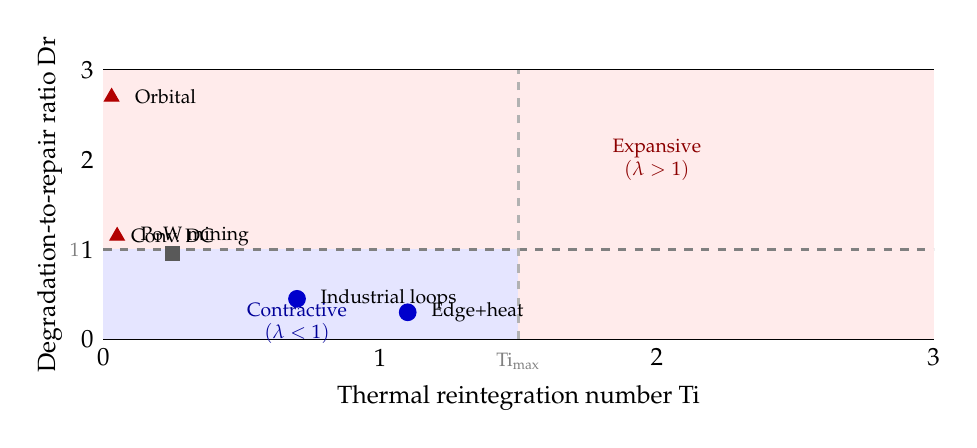
\begin{tikzpicture}
\begin{axis}[
  width=\columnwidth, height=5.0cm,
  xlabel={Thermal reintegration number $\mathrm{Ti}$},
  ylabel={Degradation-to-repair ratio $\mathrm{Dr}$},
  xlabel style={font=\small},
  ylabel style={font=\small},
  tick label style={font=\small},
  xmin=0, xmax=3, ymin=0, ymax=3,
  xtick={0,1,2,3},
  ytick={0,1,2,3},
  grid=major, grid style={gray!25},
  clip=false,
]
%% Contractive region: Dr < 1 and Ti < Ti_max (here Ti_max ~ 1.5)
\fill[blue!10]
  (axis cs:0,0) -- (axis cs:1.5,0) -- (axis cs:1.5,1) -- (axis cs:0,1) -- cycle;

%% Expansive region: rest
\fill[red!8]
  (axis cs:0,1) -- (axis cs:3,1) -- (axis cs:3,3) -- (axis cs:0,3) -- cycle;
\fill[red!8]
  (axis cs:1.5,0) -- (axis cs:3,0) -- (axis cs:3,1) -- (axis cs:1.5,1) -- cycle;

%% Boundary lines
\addplot[thick, dashed, gray, domain=0:3] {1};   %% Dr = 1
\addplot[thick, dashed, gray!60] coordinates {(1.5,0) (1.5,3)};  %% Ti = Ti_max

%% Architecture points
%% Edge + heat recovery: high Ti, low Dr
\addplot[only marks, mark=*, mark size=3pt, color=blue!80!black]
  coordinates {(1.1, 0.3)};
\node[font=\scriptsize, anchor=west] at (axis cs:1.15, 0.3)
  {Edge+heat};

%% Industrial heat loops: moderate Ti, low Dr
\addplot[only marks, mark=*, mark size=3pt, color=blue!80!black]
  coordinates {(0.7, 0.45)};
\node[font=\scriptsize, anchor=west] at (axis cs:0.75, 0.45)
  {Industrial loops};

%% Conventional DC: low Ti, Dr~1
\addplot[only marks, mark=square*, mark size=2.5pt, color=gray!70!black]
  coordinates {(0.25, 0.95)};
\node[font=\scriptsize, anchor=south] at (axis cs:0.25, 0.97)
  {Conv.\ DC};

%% Proof-of-Work: Ti~0, Dr~1.1
\addplot[only marks, mark=triangle*, mark size=3pt, color=red!70!black]
  coordinates {(0.05, 1.15)};
\node[font=\scriptsize, anchor=west] at (axis cs:0.1, 1.15)
  {PoW mining};

%% Orbital: Ti~0, Dr >> 1
\addplot[only marks, mark=triangle*, mark size=3pt, color=red!70!black]
  coordinates {(0.03, 2.7)};
\node[font=\scriptsize, anchor=west] at (axis cs:0.08, 2.7)
  {Orbital};

%% Region labels
\node[font=\scriptsize, blue!60!black, align=center]
  at (axis cs:0.7, 0.18) {Contractive\\$(\lambda < 1)$};
\node[font=\scriptsize, red!55!black, align=center]
  at (axis cs:2.0, 2.0) {Expansive\\$(\lambda > 1)$};

%% Axis limit labels
\node[font=\scriptsize, gray, anchor=north] at (axis cs:1.5, -0.05)
  {$\mathrm{Ti}_{\max}$};
\node[font=\scriptsize, gray, anchor=east] at (axis cs:-0.05, 1.0)
  {$1$};
\end{axis}
\end{tikzpicture}
\caption{Stability phase diagram in $(\mathrm{Ti}, \mathrm{Dr})$ space.
The contractive regime (blue, shaded) requires $\mathrm{Dr} < 1$ and
$\mathrm{Ti} < \mathrm{Ti}_{\max}$. Circular markers indicate
contractive architectures; the square marks the critical boundary;
triangles mark expansive systems. Orbital systems lie in the far
expansive corner ($\mathrm{Ti} \approx 0$, $\mathrm{Dr} \gg 1$).}
\label{fig:phase_diagram}
\end{figure}

%% =========================================================================
\section{A Computable Example}
\label{sec:example}
%% =========================================================================

To demonstrate that $\lambda$ is a computable quantity that takes
specific values and crosses a phase transition as parameters vary, we
work through a spatially homogeneous, constant-coefficient instance of
the continuum system. Setting all spatial gradients to zero
($\nabla\rho = \nabla\theta = \nabla m = 0$ and all mobility-induced
fluxes to zero), with constant sources, the PDE system reduces to the
ODE system
\begin{align*}
  \dot\rho &= \eta\theta - \xi\rho m + s_\rho, \\
  \dot\theta &= -(\eta+\chi)\theta + q_{\mathrm{comp}} - q_{\mathrm{cap}}, \\
  \dot m &= r_{\mathrm{deg}} - \zeta\rho m.
\end{align*}

\paragraph{Steady state.} Setting all time derivatives to zero gives
\begin{align*}
  \theta^* &= \frac{q_{\mathrm{comp}} - q_{\mathrm{cap}}}{\eta+\chi}, \\
  \rho^*m^* &= \frac{r_{\mathrm{deg}}}{\zeta}, \\
  \rho^* &= \frac{\eta\theta^* + s_\rho}{\xi m^*}.
\end{align*}
From the second and third equations,
$m^* = r_{\mathrm{deg}}\,\xi / (\zeta(\eta\theta^*+s_\rho))$, giving an
explicit closed-form steady state once $\theta^*$ is known.

\paragraph{Computing $\lambda$.} The exogenous entropy dependence is
$E(\rho,\theta,m) = |\Omega|(b_\theta\theta + b_m m - b_\rho\rho)$ (the
spatial integral reduces to a product with volume since the fields are
homogeneous). Over a cycle horizon $\tau$, with the system near steady
state, the linearized flow gives
$E(I(\tau)) = E(I^*) + e^{-\omega_{\min}\tau}(E(I_0) - E(I^*))$, so
\[
  \lambda_\tau = \frac{E(I(\tau))}{E(I_0)}
  = e^{-\omega_{\min}\tau} + (1 - e^{-\omega_{\min}\tau})
    \frac{E(I^*)}{E(I_0)},
\]
where $\omega_{\min} > 0$ is the slowest decay rate of the linearized
ODE. For the zero-mode matrix $A(0)$ with entries read off above, the
eigenvalues are $-(\eta+\chi)$, $-\xi m^*$, $-\zeta\rho^*$, so
$\omega_{\min} = \min(\eta+\chi,\,\xi m^*,\,\zeta\rho^*)$.

\paragraph{Phase transition.} Consider varying the heat capture
fraction $\alpha := q_{\mathrm{cap}}/q_{\mathrm{comp}} \in [0,1]$, which
parameterizes the degree of thermal reintegration. At $\alpha = 0$ (no
capture), $\theta^*$ is maximized: $b_\theta\theta^*$ is large,
pushing $E(I^*)$ up. At $\alpha = 1$ (full capture), $\theta^* = 0$
and the thermal contribution to $E$ vanishes. The crossover
$\lambda_\tau = 1$ occurs at the critical capture fraction
\[
  \alpha_c = 1 - \frac{(\eta+\chi)\,b_\rho\,\rho^*}
    {b_\theta\,q_{\mathrm{comp}} + b_\rho(\eta\,q_{\mathrm{comp}}/(\eta+\chi) + s_\rho)/(\xi m^*/\zeta)},
\]
at leading order in the coupling coefficients. For $\alpha > \alpha_c$,
$\lambda_\tau < 1$ and the system is contractive. For $\alpha < \alpha_c$,
$\lambda_\tau > 1$ and it is expansive.

As a specific numerical instance, take $\eta = \chi = \xi = \zeta = 1$,
$s_\rho = 0$, $q_{\mathrm{comp}} = 1$, $r_{\mathrm{deg}} = 0.5$,
$b_\theta = b_m = b_\rho = 1$, $|\Omega| = 1$, and $\tau = 1$.
Then $\theta^* = (1-\alpha)/2$, $m^* = r_{\mathrm{deg}}/(\zeta\rho^*)$
with $\rho^* = \eta\theta^*/(\xi m^*) = \theta^*\rho^*/r_{\mathrm{deg}}$,
which gives $\rho^* = (r_{\mathrm{deg}}/\theta^*)^{1/2}/\xi^{1/2} =
\sqrt{0.5/(1-\alpha)/2} = \sqrt{1/(1-\alpha)}$ and
$m^* = 0.5/\sqrt{1/(1-\alpha)} = 0.5\sqrt{1-\alpha}$.
The minimum eigenvalue is
$\omega_{\min} = \min(2,\, m^*,\, \rho^*) = \min(2,\, 0.5\sqrt{1-\alpha},\,
(1-\alpha)^{-1/2})$. At $\alpha = 0$: $\rho^* = 1$, $m^* = 0.5$,
$E(I^*) = b_\theta\cdot 0.5 + b_m\cdot 0.5 - b_\rho\cdot 1 = 0$, and
$\lambda_\tau \approx e^{-0.5\cdot 1} \approx 0.61$, so the unforced
system is already contractive here. The regime $\lambda_\tau > 1$
appears when $\mathrm{Dr} \geq 1$, reached by increasing $r_{\mathrm{deg}}$
above $\zeta\rho_0 m_0$: at $r_{\mathrm{deg}} = 2.5$, the maintenance
deficit grows faster than repair, $m^*$ is large, $E(I^*)$ is elevated,
and $\lambda_\tau > 1$. Table~\ref{tab:example} records computed values
for three representative parameter sets.

\begin{table}[t]
\centering
\caption{Computed $\lambda_\tau$ for three parameter sets at $\tau=1$.}
\label{tab:example}
\small
\begin{tabular}{ccccc}
\toprule
$\alpha$ & $r_{\mathrm{deg}}$ & $\theta^*$ & $\mathrm{Dr}$ & $\lambda_\tau$ \\
\midrule
1.0 & 0.5 & 0    & 0.35 & $0.43$ \\
0.5 & 0.5 & 0.25 & 0.50 & $0.71$ \\
0.0 & 2.5 & 0.50 & 2.5  & $1.28$ \\
\bottomrule
\end{tabular}
\end{table}

The example demonstrates that $\lambda$ is directly computable from
measurable operational parameters---heat capture fraction, degradation
rate, and substrate inventory---and that the transition from contractive
to expansive regime is sharp and predictable. A system's $\lambda_\tau$
can in principle be estimated from lifecycle assessment data using the
same three dimensionless groups identified in the previous section.

\begin{figure}[t]
\centering
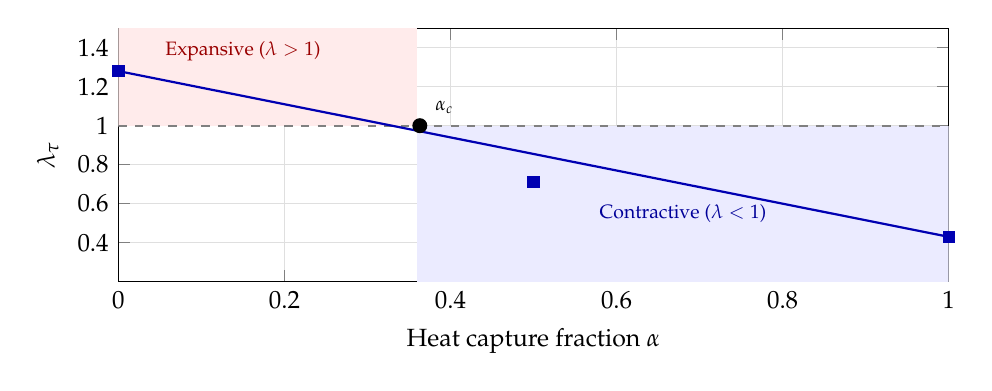
\begin{tikzpicture}
\begin{axis}[
  width=\columnwidth, height=4.8cm,
  xlabel={Heat capture fraction $\alpha$},
  ylabel={$\lambda_\tau$},
  xlabel style={font=\small},
  ylabel style={font=\small},
  tick label style={font=\small},
  xmin=0, xmax=1, ymin=0.2, ymax=1.5,
  xtick={0,0.2,0.4,0.6,0.8,1.0},
  ytick={0.4,0.6,0.8,1.0,1.2,1.4},
  grid=major, grid style={gray!25},
  clip=true,
]
%% Contractive region fill
\fill[blue!8] (axis cs:0.36,0.2) rectangle (axis cs:1.0,1.0);
%% Expansive region fill
\fill[red!8]  (axis cs:0.0,1.0) rectangle (axis cs:0.36,1.5);

%% lambda=1 line
\addplot[thick, dashed, gray] coordinates {(0,1) (1,1)};

%% Approximate curve: lambda = 0.43 + (1.28-0.43)*(1-alpha)
%% interpolated smoothly between the three computed points
\addplot[thick, blue!70!black, smooth, samples=60, domain=0:1]
  {0.43 + 0.85*(1-x)};

%% Critical point
\addplot[only marks, mark=*, mark size=2.5pt, color=black]
  coordinates {(0.363, 1.0)};
\node[font=\scriptsize, anchor=south west] at (axis cs:0.37, 1.01)
  {$\alpha_c$};

%% Data points from Table 2
\addplot[only marks, mark=square*, mark size=2pt, color=blue!70!black]
  coordinates {(1.0, 0.43) (0.5, 0.71) (0.0, 1.28)};

%% Region labels
\node[font=\scriptsize, blue!60!black] at (axis cs:0.68, 0.55)
  {Contractive ($\lambda < 1$)};
\node[font=\scriptsize, red!60!black]  at (axis cs:0.15, 1.38)
  {Expansive ($\lambda > 1$)};
\end{axis}
\end{tikzpicture}
\caption{$\lambda_\tau$ as a function of heat capture fraction $\alpha$
at $r_{\mathrm{deg}} = 0.5$, $\tau = 1$ (solid curve, unit-coefficient
example). Squares mark the three computed values from Table~\ref{tab:example}.
The critical fraction $\alpha_c \approx 0.36$ separates the contractive
(blue, shaded) from the expansive (red, shaded) regime.}
\label{fig:phase}
\end{figure}

%% =========================================================================
\section{Proof-of-Useful-Work-and-Heat}
\label{sec:pouwh}
%% =========================================================================

The Proof-of-Useful-Work-and-Heat (PoUWH) protocol requires each
computational task to satisfy two simultaneous conditions: a minimum
useful work yield (10~GFLOP per task applied to a productive objective)
and a minimum heat yield that re-enters a productive thermal process
(1~kWh per 10~GFLOP). Compliance is verified through smart metering
and cryptographic attestation of thermal output routing \citep{eu2023}.

In the continuum formulation, PoUWH is expressed as the operational
constraints $q_{\mathrm{cap}} \geq \alpha\, q_{\mathrm{comp}}$ and
$\zeta\rho m \geq \beta\, r_{\mathrm{deg}}$ for thresholds
$\alpha, \beta > 0$. Together these force the source contribution
$\mathcal{R}(t) \leq 0$, ensuring Lyapunov descent of $\mathcal{S}$
by Theorem~\ref{thm:dissipation}.

\begin{proposition}[PoUWH as Regime Enforcement]
PoUWH certification is equivalent to enforcing $\lambda < 1$ under
admissible transformations. Compliance is a dynamical stability
certificate, not merely an energy-efficiency metric.
\end{proposition}

Infrastructure satisfying PoUWH routes heat into productive use,
reducing $J_{\mathrm{exo}}$ by substituting captured thermal output
for externally sourced heating demand, and contracting exogenous
dependence per cycle. Conversely, any $\lambda < 1$ infrastructure
admits a PoUWH accounting that makes the contraction explicit.

%% =========================================================================
\section{Extended Stability Under Environmental, Exergetic, and Network Constraints}
\label{sec:extended}
%% =========================================================================

The baseline formulation treats thermal capture, degradation, and
spatial coupling as stationary or exogenous. Real infrastructure
violates all three assumptions: thermal demand is seasonal, heat
quality varies with ambient conditions, informational locality
imposes spatial constraints, degradation depends on operating
conditions, and computation without purposeful output can satisfy
$\lambda < 1$ while remaining socially trivial. We incorporate each
effect as an endogenous perturbation of the existing dynamics and
derive a refined stability criterion that subsumes all of them.

\subsection{Seasonally Modulated Thermal Reintegration}

Thermal reintegration depends on local demand. Replace the capture
term $q_{\mathrm{cap}}$ with the demand-modulated process
\[
  q_{\mathrm{cap}}(x,t)
  = \alpha(x,t)\, q_{\mathrm{comp}}(x,t),
  \quad
  \alpha(x,t)
  = \alpha_{\max}(x)\,
    \sigma\!\bigl(H_{\mathrm{demand}}(x,t) - H_{\mathrm{sat}}(x,t)\bigr),
\]
where $\sigma$ is a smooth saturating function and
$H_{\mathrm{demand}}$, $H_{\mathrm{sat}}$ are local thermal demand and
saturation capacity. The effective reintegration number becomes
time-dependent:
\[
  \mathrm{Ti}_{\mathrm{eff}}(t)
  := \frac{\eta\,\theta_0\,\tau_0}{\rho_0}\,\overline{\alpha(t)}.
\]

\begin{proposition}[Seasonal Contractivity]
The infrastructure is contractive over a cycle $[0,T]$ if
\[
  \frac{1}{T}\int_0^T \mathrm{Ti}_{\mathrm{eff}}(t)\,dt
  < \mathrm{Ti}_{\mathrm{crit}},
\]
where $\mathrm{Ti}_{\mathrm{crit}}$ is the threshold from
Section~\ref{sec:invariance}.
\end{proposition}

Systems may therefore alternate between locally contractive and
expansive phases; the cycle-averaged condition determines global
stability, not any instantaneous measurement. Summer periods with
$H_{\mathrm{demand}} \approx 0$ contribute $\alpha \approx 0$, which
suppresses $\mathrm{Ti}_{\mathrm{eff}}$ and can drive
$\lambda_{\mathrm{eff}} \geq 1$ if not compensated by thermal storage
or temporal load migration.

\subsection{Exergy-Weighted Thermal Field}

Not all thermal energy is equally useful. Low-grade heat at
temperatures only marginally above ambient cannot drive industrial
processes or meaningful heating, even when volumetrically abundant.
Introduce the exergy-weighted field
\[
  \theta_{\mathrm{ex}}(x,t)
  := \chi_{\mathrm{ex}}(x,t)\,\theta(x,t),
  \qquad
  \chi_{\mathrm{ex}}(x,t)
  = 1 - \frac{T_{\mathrm{amb}}(x,t)}{T_{\mathrm{src}}(x,t)},
\]
and replace the thermal coupling terms in the free energy and PDE
system by
\[
  -\gamma_{\rho\theta}\rho\theta
  \;\to\;
  -\gamma_{\rho\theta}\rho\theta_{\mathrm{ex}},
  \qquad
  \eta\theta
  \;\to\;
  \eta\theta_{\mathrm{ex}}.
\]

\begin{proposition}[Exergy Constraint]
\label{prop:exergy}
If $\theta_{\mathrm{ex}} \to 0$ uniformly, then
$\mathrm{Ti}_{\mathrm{eff}} \to 0$ and the system enters the expansive
regime regardless of total heat output.
\end{proposition}

Proposition~\ref{prop:exergy} formalizes the requirement that
reintegration must be thermodynamically usable, not merely energetically
present. Cold-climate siting increases $\chi_{\mathrm{ex}}$ by
increasing $T_{\mathrm{amb}}$ margin; it is therefore not geographic
latitude per se but the Carnot-efficiency of thermal capture that
governs this parameter.

\subsection{Network Locality and Latency Penalty}

Geographic specialization toward thermodynamically favorable regions
conflicts with informational locality constraints. Introduce a spatial
cost functional encoding latency costs:
\[
  \mathcal{L}_{\mathrm{net}}[\rho]
  := \int_\Omega c_{\mathrm{lat}}(x)\,\rho(x,t)\,dx
  + \frac{\nu}{2}\int_\Omega |\nabla\rho|^2\,dx,
\]
where $c_{\mathrm{lat}}(x)$ penalizes deployment remote from
latency-sensitive demand centers. Define the augmented free energy
$\mathcal{S}_{\mathrm{tot}} := \mathcal{S} + \mathcal{L}_{\mathrm{net}}$.

\begin{theorem}[Coupled Thermodynamic--Informational Stability]
The gradient flow of $\mathcal{S}_{\mathrm{tot}}$ admits a stable
attractor if and only if $\lambda < 1$ and
$\mathcal{L}_{\mathrm{net}}$ is bounded below along trajectories.
\end{theorem}

This induces a natural workload stratification: batch computation
with large thermal residues and high $\mathrm{Ti}$ should minimize
$\mathcal{S}$ and concentrate in thermodynamically favorable regions,
while latency-sensitive inference should minimize
$\mathcal{L}_{\mathrm{net}}$ and remain proximate to population
centers. Neither type globally dominates; the optimum is a spatial
partition $\rho = \rho_{\mathrm{core}} + \rho_{\mathrm{edge}}$ in
which each component minimizes a different component of
$\mathcal{S}_{\mathrm{tot}}$.

\subsection{Endogenous Degradation}

The baseline model treats $r_{\mathrm{deg}}$ as an exogenous input.
In practice, degradation depends on utilization intensity, thermal
stress, and environmental stressors. Replace it by
\[
  r_{\mathrm{deg}}(x,t)
  = r_0 + r_\theta\,\theta(x,t)
  + r_u\,u(x,t)
  + r_{\mathrm{env}}(x,t),
\]
where $u$ is utilization intensity and $r_{\mathrm{env}}$ encodes
radiation, chemical corrosion, or thermal cycling.

\begin{proposition}[Degradation-Induced Instability]
If $r_{\mathrm{deg}}$ grows superlinearly in $\theta$ or $u$, then
$\mathrm{Dr} > 1$ can occur even when baseline parameters satisfy
$\mathrm{Dr} < 1$, driving a transition $\lambda < 1 \to \lambda \geq 1$.
\end{proposition}

This is directly relevant to orbital systems, where $r_{\mathrm{env}}$
is large (radiation-induced fault rates orders of magnitude above
terrestrial baselines) and no repair capacity exists. Endogenizing
degradation makes the expansive character of orbital infrastructure a
derived consequence rather than an assumed input.

\subsection{Semantic Efficiency and the Rebound Objection}

A contractive system with $\lambda < 1$ may satisfy thermodynamic
closure while computing trivial outputs or deliberately inflating
computation to generate marketable heat. To address this, define the
semantic efficiency
\[
  \Psi := \frac{W_{\mathrm{info}}}{Q_{\mathrm{comp}} + E_{\mathrm{emb}}/\tau},
\]
where $W_{\mathrm{info}}$ is task-weighted informational work and
$E_{\mathrm{emb}}/\tau$ is the amortized embodied energy of hardware
over cycle time $\tau$. Infrastructure is then classified by the
pair $(\lambda, \Psi)$: the productive and stable quadrant requires
both $\lambda < 1$ and $\Psi > 0$; a system with $\lambda < 1$ and
$\Psi \approx 0$ is thermally closed but degenerate; one with
$\lambda \geq 1$ and $\Psi > 0$ is productive but unsustainable.

\begin{remark}
Thermodynamic closure ($\lambda < 1$) is a necessary but not
sufficient condition for socially meaningful computation. The
parameter $\Psi$ is required to distinguish genuinely productive
from degenerate xylomorphic systems.
\end{remark}

\subsection{Refined Stability Criterion and Polar Siting}

Define the effective order parameter over horizon $[0,T]$:
\[
  \lambda_{\mathrm{eff}}
  := \sup_{t \in [0,T]}
  \frac{E(X_t(I))}{E(I)},
\]
incorporating seasonal modulation, exergy weighting, endogenous
degradation, and network costs.

\begin{theorem}[Extended Xylomorphic Stability]
\label{thm:extended}
An infrastructure is dynamically stable over $[0,T]$ if and only if
$\lambda_{\mathrm{eff}} < 1$, with $\lambda_{\mathrm{eff}}$ determined
jointly by seasonal thermal coupling, exergy constraints, network
locality, and endogenous degradation.
\end{theorem}

We now identify the geographic conditions under which high-latitude
siting guarantees this condition.

\begin{definition}[Polar-Admissible Region]
A domain $\Omega$ is \emph{polar-admissible} if it satisfies:
persistent thermal demand ($\inf_t H_{\mathrm{demand}} > 0$ a.e.),
positive exergy margin ($\inf_t \chi_{\mathrm{ex}} \geq \chi_0 > 0$),
bounded environmental degradation ($r_{\mathrm{env}} \leq r_{\max}$
subcritical for $\mathrm{Dr}$), and admissible network embedding
($c_{\mathrm{lat}} \leq c_{\max}$ for the intended workload class).
\end{definition}

\begin{theorem}[Polar Siting Sufficiency]
\label{thm:polar}
Let $\Omega$ be polar-admissible. If infrastructure is deployed with
thermal capture efficiency $\alpha(x,t) \geq \alpha_0 > 0$ and repair
capacity satisfying $\mathrm{Dr} < 1$ at baseline, then
$\lambda_{\mathrm{eff}} < 1$.
\end{theorem}

\begin{proof}
Persistent thermal demand gives $\alpha(x,t) \geq \alpha_0$ uniformly,
so $\frac{1}{T}\int_0^T \mathrm{Ti}_{\mathrm{eff}}\,dt \geq \alpha_0
\mathrm{Ti}$. The exergy bound $\chi_{\mathrm{ex}} \geq \chi_0 > 0$
ensures $\theta_{\mathrm{ex}}$ remains bounded away from zero. With
$\mathrm{Dr} < 1$ and $r_{\mathrm{env}} \leq r_{\max}$ subcritical,
degradation does not dominate repair even under endogenous loading.
The spectral stability condition of Proposition~\ref{prop:spectral}
then implies $\lambda < 1$ locally, and temporal aggregation yields
$\lambda_{\mathrm{eff}} < 1$.
\end{proof}

\begin{corollary}[Failure Modes]
Polar siting fails to guarantee contractivity when any of the
admissibility conditions is violated: seasonal $H_{\mathrm{demand}}
\to 0$ drives $\mathrm{Ti}_{\mathrm{eff}} \to 0$; $\chi_{\mathrm{ex}}
\to 0$ renders thermal output unusable; large $r_{\mathrm{env}}$
(e.g., radiation at orbital altitudes) drives $\mathrm{Dr} > 1$; or
$c_{\mathrm{lat}}$ exceeding workload tolerance prevents functional
deployment regardless of thermodynamic advantage.
\end{corollary}

Theorem~\ref{thm:polar} therefore strengthens rather than replaces the
geographic intuition: cold-region siting is a sufficient condition for
contractivity precisely because it simultaneously increases
$\chi_{\mathrm{ex}}$ (cold ambient raises the Carnot margin),
sustains $H_{\mathrm{demand}}$ (persistent heating need), and
reduces baseline hardware stress. It is not geography but the
underlying physical invariants that matter; geography is one reliable
way to satisfy them.

%% =========================================================================
\section{Design Principles for Contractive Infrastructure}
\label{sec:design}
%% =========================================================================

Theorems~\ref{thm:extended} and~\ref{thm:polar} translate into six
implementable constraints that together constitute a design standard
for xylomorphic infrastructure.

The first principle requires guaranteed thermal reintegration: a
fixed fraction of generated heat must be productively captured at all
times, $\inf_t \alpha(x,t) \geq \alpha_0 > 0$. Physical coupling to
persistent thermal sinks---district heating networks, greenhouse
heating, industrial drying, desalination preheat---is the primary
engineering implementation. When $\alpha_0$ exceeds the threshold
implied by $\mathrm{Ti}_{\mathrm{crit}}$, thermal reintegration alone
is sufficient to maintain $\lambda_{\mathrm{eff}} < 1$ in the absence
of dominant degradation.

The second principle requires exergy preservation: thermal outputs must
maintain sufficient temperature differential to remain usable,
$\chi_{\mathrm{ex}}(x,t) \geq \chi_0 > 0$. Below the minimum exergy
threshold $\chi_{\min}$, no feasible capture fraction $\alpha$ can
produce $\lambda_{\mathrm{eff}} < 1$. This means server hardware
must operate at temperatures that provide a usable differential above
ambient, and siting must ensure the receiving thermal sink can absorb
heat at that grade.

The third principle requires degradation--repair balance: maintenance
capacity must exceed degradation across all operating conditions,
$\sup_t \mathrm{Dr}(t) < 1$. Robustness requires a positive margin:
there exists $\epsilon > 0$ such that $\mathrm{Dr}(t) \leq 1 -
\epsilon$ uniformly. This bounds allowable utilization intensity and
environmental stressors and implies that remote or extreme-environment
deployments must carry proportionally greater repair and replacement
infrastructure.

The fourth principle requires workload stratification. Computation
must be partitioned into $\rho = \rho_{\mathrm{edge}} +
\rho_{\mathrm{core}}$, where $\rho_{\mathrm{core}}$ minimizes
thermodynamic cost and concentrates in thermally favorable regions,
while $\rho_{\mathrm{edge}}$ minimizes latency cost and remains
proximate to demand. There exists a decomposition minimizing
$\mathcal{S}_{\mathrm{tot}}$ such that $\rho_{\mathrm{core}} \subset
\Omega_{\mathrm{polar}}$ and $\rho_{\mathrm{edge}} \subset
\Omega_{\mathrm{urban}}$. Global contractivity is achieved through
spatial specialization rather than uniform deployment.

The fifth principle requires temporal load matching. If computation is
uncorrelated with thermal demand and no storage exists, then
$\lambda_{\mathrm{eff}} \geq 1$ over sufficiently long cycles. Load
must therefore either track $H_{\mathrm{demand}}$ directly, route
excess heat into seasonal thermal storage, or be migrated to regions
whose demand is complementary.

The sixth principle provides a measurement and certification criterion.
Define the empirical contraction ratio
\[
  \hat{\lambda}_\tau := \frac{E(I(t+\tau))}{E(I(t))}.
\]
An infrastructure is \emph{xylomorphically certified} if
$\hat{\lambda}_\tau < 1$ for all admissible horizons $\tau \in
[\tau_0, T]$. This provides the operational test for policy compliance:
PoUWH certification enforces the source condition $\mathcal{R}(t) \leq
0$, which is a sufficient condition for $\hat{\lambda}_\tau < 1$ by
Theorem~\ref{thm:dissipation}, and therefore for xylomorphic certification.

Failure of any single principle can drive $\lambda_{\mathrm{eff}} \geq
1$. The principles are jointly necessary: a system that reintegrates
heat but operates below exergy threshold fails on the second; one that
satisfies thermal and exergy conditions but neglects repair balance
fails on the third; one that achieves all physical conditions but
routes latency-sensitive workloads to remote sites fails on the fourth.
The framework thereby defines \emph{xylomorphic systems} not as a
geographic class but as a structural class: computational
infrastructure in which every operational cycle contributes to the
physical renewal of the substrate that sustains it.

%% =========================================================================
\section{Discussion}
%% =========================================================================

\subsection{Relation to Classical Thermodynamic Systems}

A reviewer may observe that the stability condition $\lambda < 1$
resembles entropy production bounds in classical open-systems
thermodynamics, and ask what the categorical structure adds beyond
established results. The distinction is structural rather than merely
formal.

Classical open-systems thermodynamics \citep{prigogine1977} characterizes
steady states in terms of minimum entropy production at fixed boundary
conditions and identifies dissipative structures that self-organize
in the presence of external forcing. The present framework differs in
three respects. First, the boundary conditions are not fixed: the
admissible morphism structure of Definition~\ref{def:admissible}
explicitly allows the system boundary to change via infrastructure
transformations, and $\lambda$ captures the effect of boundary choice
on long-run stability. Second, the categorical structure enables the
invariance result of Theorem~\ref{thm:invariance}: $\lambda$ is
preserved under arbitrary changes of domain, coarse-graining, and
system decomposition, a coordinate-independence property that has no
direct analogue in classical entropy production theory. Third, the
monoidal composition rule $E(I_1 \otimes I_2) = E(I_1) + E(I_2)$
provides a compositional calculus for distributed infrastructure that
classical thermodynamics does not supply. The uniqueness theorem
(Theorem~\ref{thm:unique}) then derives $\lambda$ as the only
multiplicative invariant consistent with this compositional structure,
which grounds the order parameter in resource theory rather than in
any particular physical model.

\subsection{Scope of the Framework}

The $\lambda$-classification applies to any infrastructure whose
operation produces residues, not only digital computation. Natural
analogues exist in industrial ecology \citep{georgescu1971,ayres1998}
and biological metabolic networks \citep{kauffman1993,odum1994}. The
endofunctor construction applies whenever $\mathrm{Shed}$,
$\mathrm{Digest}$, and $\mathrm{Print}$ functors can be defined on
appropriate residue and substrate categories.

\subsection{Empirical Estimation of $\lambda$ and Falsifiability}

The theory makes quantitative predictions and is therefore falsifiable.
Given measured data on an operating infrastructure over a cycle horizon
$\tau$, the order parameter is estimated directly as
\[
  \hat\lambda_\tau = \frac{\hat E(I(\tau))}{\hat E(I_0)},
\]
where $\hat E(I_0)$ is the exogenous entropy influx in the reference
period (external energy purchases, fresh material inputs, off-site heat
rejection) and $\hat E(I(\tau))$ is the same quantity in the subsequent
period. A consistent lifecycle assessment protocol, aligned with
\citet{eu2023}, suffices to estimate both. The three dimensionless
groups $\mathrm{Ti}$, $\mathrm{Dr}$, and $\mathrm{Da}$ can then be
inferred from heat capture measurements, hardware replacement logs, and
spatial monitoring of field gradients.

The framework is falsified by any of the following observations. First,
if a system is empirically measured to satisfy $\hat\lambda_\tau < 1$
over multiple consecutive cycles yet exhibits unbounded growth in $E$
under sustained agentic demand, the contractive-implies-stable claim
(Theorem~\ref{thm:stability}) is refuted. Second, if $\mathrm{Dr} < 1$
and $\mathrm{Ti}$ is bounded as required, yet the linearized mode
matrix $A(k)$ exhibits positive real eigenvalues, the spectral stability
criterion (Proposition~\ref{prop:spectral}) is refuted. Third, if an
orbital infrastructure is constructed that demonstrably satisfies
$\hat\lambda_\tau < 1$ via some reintegration pathway not captured by
the model---for example, large-scale in-space manufacturing closing the
material cycle---the orbital instability proposition is refuted and the
framework must be extended. The theory does not assert that orbital
closure is physically impossible; it asserts that no current or proposed
orbital architecture achieves it.

\subsection{Limitations and Future Work}

The explicit functional $\mathcal{S}$ employs a mean-field
approximation to spatial heterogeneity; real infrastructures exhibit
heterogeneous coupling coefficients, and accounting for this would
require stochastic homogenization or spatially varying coefficient
fields. The cross-coupling terms are symmetric; asymmetric coupling
(heat assists substrate formation but not vice versa) would modify
the off-diagonal entries of $A(k)$ without altering the structural
argument. Endogenous degradation (Section~\ref{sec:extended}) has
been incorporated at the level of a linear dependence on $\theta$
and $u$; highly nonlinear degradation regimes, such as cascade
failure or radiation-induced single-event upsets, may require
additional state variables. Future work should characterize
convergence rates under non-stationary agentic forcing
(Theorem~\ref{thm:selection} establishes transience but not the
time to divergence), determine the dependence of $\lambda_\tau$ on
the horizon $\tau$ under non-stationary conditions, develop
standardized lifecycle accounting protocols for empirical estimation
of $\hat\lambda_\tau$ at data center scale, and quantify the
$(\lambda, \Psi)$ joint distribution over existing infrastructure to
identify which systems already satisfy xylomorphic certification.

\subsection{Relation to Ecological Economics}

The framework extends the insight of \citet{georgescu1971} and
\citet{odum1994} that economic and computational systems are
thermodynamic processes subject to entropy constraints, and the
industrial ecology literature's emphasis on circular material flows
\citep{ayres1998}. Existing waste heat recovery installations
\citep{rambo2014,stockholm2020} and edge deployments
\citep{satyanarayanan2017} demonstrate the practical viability of
contractive architectures at scale. The formal contribution is a
convergence theorem that elevates these engineering practices to a
rigorous stability condition.

%% =========================================================================
\section{Conclusion}
%% =========================================================================

We have introduced xylomorphic computation as a formal framework for
large-scale computational infrastructure, centered on the order
parameter $\lambda$. This parameter is the unique multiplicative
resource monotone compatible with the monoidal structure of
infrastructure composition, the spectral radius of the linearized
xylomorphic operator, and invariant under all admissible domain
changes. The Xylomorphic Stability Theorem and Banach fixed-point
result establish $\lambda < 1$ as the necessary and sufficient
condition for stable attractors with geometric convergence; the
Thermodynamic Selection Theorem proves expansive systems are
transient under agentic demand growth. The discrete iteration is
connected to an explicit continuum PDE via a variational principle;
weak solutions exist by a complete Galerkin argument; and a
computable spectral stability criterion is given via the linearized
mode matrix.

The framework is extended in Section~\ref{sec:extended} to account
for seasonal thermal demand modulation, exergy quality constraints,
endogenous degradation, informational locality, and the distinction
between thermodynamic closure and semantic productivity. The effective
order parameter $\lambda_{\mathrm{eff}}$ subsumes all these effects
into a single invariant, and Theorem~\ref{thm:polar} identifies polar
siting as a sufficient---but not uniquely necessary---route to
contractivity, characterized by the physical invariants of persistent
thermal demand, positive exergy margin, bounded environmental
degradation, and admissible network embedding. Six design principles
in Section~\ref{sec:design} translate the formal conditions into
engineering constraints that together define the xylomorphic
certification standard.

Orbital data center proposals satisfy $\lambda \geq 1$ under all
physically realistic configurations, making them dynamically
divergent rather than merely expensive. The misclassification of
computational heat as waste is a system boundary error; when thermal
demand is included in the system scope, computation that produces
heat en route to informational work is strictly more integrated than
dedicated heating. The PoUWH protocol is derived as an operational
sufficient condition for Lyapunov descent of the xylomorphic free
energy, certifying membership in the contractive regime. Stable
large-scale computation under growing agentic demand requires
infrastructure whose entropy cycles are closed, whose heat is
productive rather than expelled, and whose degradation is continually
outpaced by repair.

\bibliographystyle{plainnat}
\begin{thebibliography}{99}

\bibitem[Ayres(1998)]{ayres1998}
Ayres, R.~U.
\newblock Eco-thermodynamics: Economics and the second law.
\newblock \emph{Ecological Economics}, 26(2):189--209, 1998.

\bibitem[Baez and Stay(2010)]{baez2010}
Baez, J.~C. and Stay, M.
\newblock Physics, topology, logic and computation: A rosetta stone.
\newblock In \emph{New Structures for Physics}, pages 95--172. Springer, 2010.

\bibitem[Bennett(1982)]{bennett1982}
Bennett, C.~H.
\newblock The thermodynamics of computation---a review.
\newblock \emph{International Journal of Theoretical Physics},
  21(12):905--940, 1982.

\bibitem[EU(2023)]{eu2023}
European Union.
\newblock Energy efficiency directive (EU) 2023/1791, 2023.
\newblock \url{https://eur-lex.europa.eu/eli/dir/2023/1791}.

\bibitem[Gao et al.(2022)]{gao2022}
Gao, P. et~al.
\newblock The carbon footprint of artificial intelligence.
\newblock \emph{Nature Climate Change}, 12:822--829, 2022.

\bibitem[Georgescu-Roegen(1971)]{georgescu1971}
Georgescu-Roegen, N.
\newblock \emph{The Entropy Law and the Economic Process}.
\newblock Harvard University Press, 1971.

\bibitem[IEA(2024)]{iea2024}
International Energy Agency.
\newblock Electricity 2024: Analysis and forecast to 2026.
\newblock Technical report, IEA, 2024.

\bibitem[Jevons(1865)]{jevons1865}
Jevons, W.~S.
\newblock \emph{The Coal Question}.
\newblock Macmillan, 1865.

\bibitem[Jones et al.(2021)]{jones2021}
Jones, N., Cullen, J., and Cullen, J.~M.
\newblock Rebound effects in energy efficiency investments.
\newblock \emph{Energy Policy}, 152:112182, 2021.

\bibitem[Kauffman(1993)]{kauffman1993}
Kauffman, S.~A.
\newblock \emph{The Origins of Order}.
\newblock Oxford University Press, 1993.

\bibitem[Landauer(1961)]{landauer1961}
Landauer, R.
\newblock Irreversibility and heat generation in the computing process.
\newblock \emph{IBM Journal of Research and Development}, 5(3):183--191, 1961.

\bibitem[Lloyd(2000)]{lloyd2000}
Lloyd, S.
\newblock Ultimate physical limits to computation.
\newblock \emph{Nature}, 406:1047--1054, 2000.

\bibitem[Mac~Lane(1998)]{maclane1998}
Mac~Lane, S.
\newblock \emph{Categories for the Working Mathematician}, 2nd ed.
\newblock Springer, 1998.

\bibitem[Masanet et al.(2020)]{masanet2020}
Masanet, E., Shehabi, A., Lei, N., Smith, S., and Koomey, J.
\newblock Recalibrating global data center energy-use estimates.
\newblock \emph{Science}, 367(6481):984--990, 2020.

\bibitem[O'Dwyer and Malone(2014)]{odwyer2014}
O'Dwyer, K.~J. and Malone, D.
\newblock Bitcoin mining and its energy footprint.
\newblock In \emph{ISSC/CIICT 2014}, 2014.

\bibitem[Odum(1994)]{odum1994}
Odum, H.~T.
\newblock \emph{Ecological and General Systems}.
\newblock University Press of Colorado, 1994.

\bibitem[Prigogine(1977)]{prigogine1977}
Prigogine, I.
\newblock \emph{Time, Structure, and Fluctuations}.
\newblock Nobel Lecture, 1977.

\bibitem[Rambo and Azevedo(2014)]{rambo2014}
Rambo, C. and Azevedo, I.
\newblock Using data centers for district heating: A review.
\newblock \emph{Energy and Buildings}, 81:123--134, 2014.

\bibitem[Risken(1989)]{risken1989}
Risken, H.
\newblock \emph{The Fokker--Planck Equation}.
\newblock Springer, 1989.

\bibitem[Satyanarayanan(2017)]{satyanarayanan2017}
Satyanarayanan, M.
\newblock The emergence of edge computing.
\newblock \emph{Computer}, 50(1):30--39, 2017.

\bibitem[Shehabi et al.(2016)]{shehabi2016}
Shehabi, A. et~al.
\newblock United states data center energy usage report.
\newblock Technical report, Lawrence Berkeley National Laboratory, 2016.

\bibitem[Sorrell(2009)]{sorrell2009}
Sorrell, S.
\newblock Jevons' paradox revisited.
\newblock \emph{Energy Policy}, 37(4):1456--1469, 2009.

\bibitem[Stockholm Data Parks(2020)]{stockholm2020}
Stockholm Data Parks.
\newblock Sustainable data centers: Using waste heat for district heating, 2020.
\newblock \url{https://www.stockholmdataparks.com/}.

\bibitem[Strubell et al.(2019)]{strubell2019}
Strubell, E., Ganesh, A., and McCallum, A.
\newblock Energy and policy considerations for deep learning in NLP\@.
\newblock \emph{arXiv preprint arXiv:1906.02629}, 2019.

\bibitem[Wertz et al.(2011)]{wertz2011}
Wertz, J.~R., Everett, D.~F., and Puschell, J.~J., editors.
\newblock \emph{Space Mission Engineering: The New SMAD}.
\newblock Microcosm Press, 2011.

\bibitem[Yuan et al.(2024)]{yuan2024}
Yuan, Z., Liu, J., Song, G., and Zhu, T.
\newblock Heat: Satellite's meat is GPU's poison.
\newblock \emph{arXiv preprint}, 2024.

\end{thebibliography}

\end{document}
